\documentclass[slovene,11pt,a4paper]{article}
\usepackage[margin=1.8cm,bottom=3cm,foot=1.5cm]{geometry}
\usepackage{amsmath}
\usepackage{booktabs}
\usepackage{float}
\usepackage{graphicx}
\usepackage{gensymb}
\usepackage{geometry}
\usepackage{changepage}
\usepackage{subcaption}
\usepackage{multirow}
\usepackage{blindtext}
\usepackage{hyperref}
\usepackage[version=4]{mhchem}
\usepackage[slovene]{babel}
\pagenumbering{gobble}
\renewcommand{\contentsname}{\centering Contents}

\begin{document}

\title{7. naloga - Naključna števila in integracije z metodo Monte Carlo}
\author{Tadej Lozej 28201055}
\maketitle
\begin{center}
Modelska analiza 1 \\
\bigskip
Predavatelj: prof. dr. Simon Širca \\
Asistent: doc. dr. Miha Mihovilovič
\end{center}

\newpage

\tableofcontents

\newpage

\section{Uvod}

\pagenumbering{arabic}

V nalogi smo se spoznali z uporabnostjo metode Monte Carlo. To je metoda v kateri z naključnim generiranjem števil in pravilnim obravnavanjem dogodkov, ki jih ta naključna števila diktirajo, pridemo do uporabnih rezultatov. Pri prvi nalogi smo izračunali maso in vztrajnostni moment zanimivega telesa. V drugi nalogi smo izračunali verjetnost za pobeg žarkov $\gamma$, v zadnji nalogi pa odbojnost in propustnost nevronskega reflektorja.

\section{Zanimivo telo}

Telesu, ki ga omejuje ploskev

\begin{equation}
\sqrt{|x|} + \sqrt{|y|} + \sqrt{|z|} = 1,
\end{equation}
smo s pomočjo Monte Carlo metode izračunali maso ter vztrajnostni moment. Na sliki 1 je prikazano zanimivo telo omejeno z ploskvijo, ki jo podaja enačba 1. Iz slike je razvidno, da je telo simetrično.

\begin{figure}[h!]
\centering
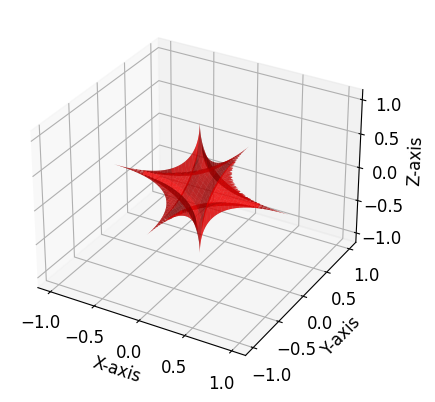
\includegraphics[width=8cm]{telo1.png}
\caption{Zanimivo telo.}
\end{figure}

Objekt lahko zajamemo v kocko z stranico dolžine dva okrog koordinatnega izhodišča. Po tej kocki nato naključno izbiramo točke z generatorjem naključnih števil v programskem jeziku \texttt{Python} z modulom \texttt{numpy.random}. Za vsako izžrebano točko $(x_i, y_i, z_i)$ pogledamo ali ustreza neenačbi

\begin{equation}
\sqrt{|x_i|} + \sqrt{|y_i|} + \sqrt{|z_i|} < 1
\end{equation}
oz. če se nahaja v telesu ali ne. Recimo, da izžrebamo vse skupaj $N$ točk. Za vsako iskano količino $\theta$ telesa bo enačba za oceno le-te oblike

\begin{equation}
\hat{\theta} = \frac{1}{N} \sum_{i=1}^N g(x_i),
\end{equation}
kjer je $g(x)$ neka funkcija s katero pridemo do želene količine. Za dovolj velike $N$ bo ocena napake enaka

\begin{equation}
\hat{\sigma_{\theta}} = \frac{\sum_{i=1}^N g(x_i)^2 - \left( \sum_{i=1}^N g(x_i) \right)^2}{N^{3/2}}.
\end{equation}
Tako bomo v naslednjih podpoglavjih ocenili maso in vztrajnostni moment telesa.

\subsection{Masa telesa}

Maso telesa izračunamo po formuli

\begin{equation}
m = \frac{V_k}{N} \sum_{i=1}^N \Delta_i \rho(r_i),
\end{equation}
kjer je $V_k = 8$ volumen kocke v katero smo telo objeli, $N$ število izžrebanih naključnih točk, $\Delta_i$ ima vrednost $1$, če se točka nahaja v telesu oz. reši neenačbo (2) ter vrednost $0$ sicer in $\rho(r_i)$ gostota v ročki $r_i = (x_i, y_i, z_i)$. Napaka za izračunano maso je

\begin{equation}
\sigma_m = \frac{V_k}{N^{3/2}} \sqrt{N\sum_{i=1}^N \Delta_i^2 \rho^2(r_i) - 
\left( \sum_{i=1}^N \Delta_i \rho(r_i) \right)^2}.
\end{equation}

\subsubsection{Konstantna gostota}

Poglejmo si rezultate za konstantno gostoto $\rho(x,y,z)=1$. Na sliki 2 so prikazane ocene za maso telesa v odvisnosti od števila izžrebanih točk $N$.

\begin{figure}[h!]
\centering
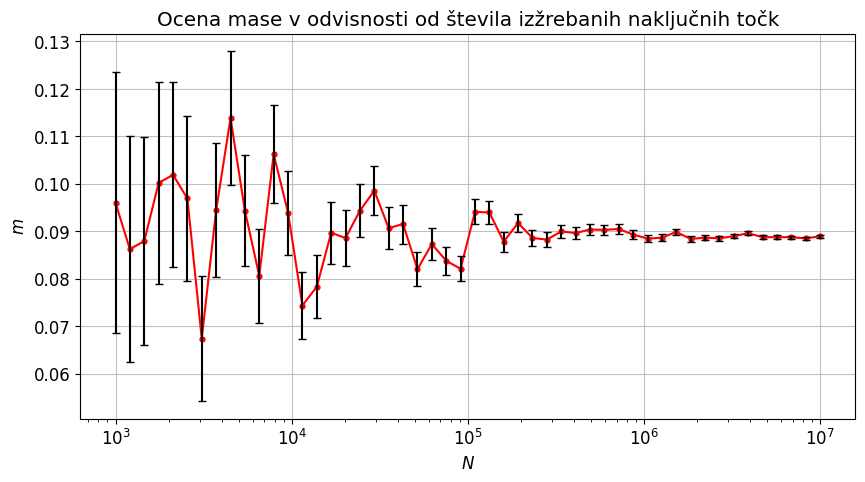
\includegraphics[width=13cm]{telo2.png}
\caption{Ocena za maso telesa v odvisnosti od števila izžrebanih točk $N$.}
\end{figure}
Vidimo, da se seveda z številom izžrebanih točk načeloma naša natančnost ocene izboljšuje. Pri $N=10^7$ točkah dobimo rezultat za oceno mase

\[
m = (88.9 \pm 0.3) \cdot 10^{-3}.
\]


\subsubsection{Gostota odvisna od radija}

Uvedimo gostoto kot funkcijo radija

\begin{equation}
\rho(r) = r^p,
\end{equation}
kjer je $r$ oddaljenost od koordinatnega izhodišča $r = \sqrt{x^2+y^2+z^2}$ ter $p$ prosti parameter. Pri številu $N=10^7$ izžrebanih točk si poglejmo kako se masa telesa spreminja z vrednostjo parametra $p$. Na sliki 3 je prikazana ocena mase v odvisnosti od vrednosti parametra p pri $N=10^7$ naključnih točkah. Vidimo, da vrednost ocene za maso precej hitro pade, saj je večino volumna telesa blizu koordinatnega izhodišča, kjer je gostota zmeraj manjša za večje vrednosti $p$.

\begin{figure}[h!]
\centering
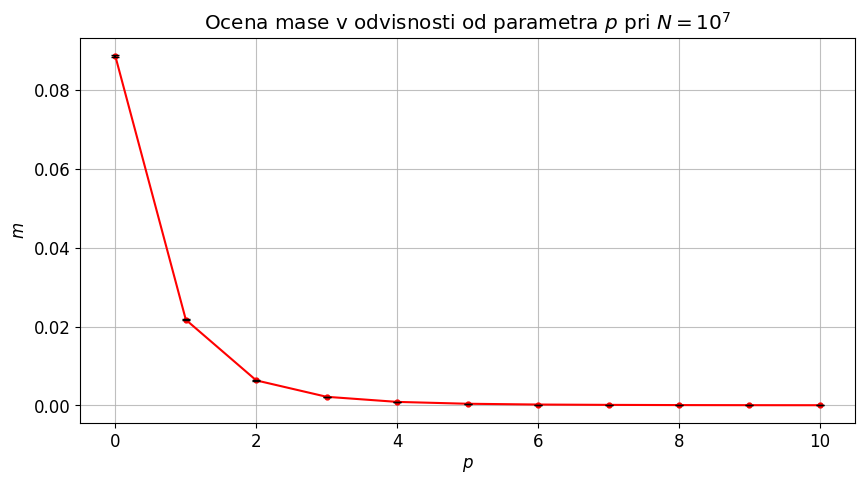
\includegraphics[width=13cm]{telo4.png}
\caption{Ocena mase v odvisnosti od vrednosti parametra p pri $N=10^7$ naključnih točkah.}
\end{figure}


\subsection{Vztrajnostni moment}

Vztrajnostni moment telesa izračunamo po formuli

\begin{equation}
J_k = \frac{V_k}{N} \sum_{i=1}^N \Delta_i d_{k,i}^2 \rho(r_i),
\end{equation}
kjer je $V_k = 8$ volumen kocke v katero smo telo objeli, $N$ število izžrebanih naključnih točk, $\Delta_i$ ima vrednost $1$, če se točka nahaja v telesu oz. reši neenačbo (2) ter vrednost $0$ sicer in $\rho(r_i)$ gostota v ročki $r_i = (x_i, y_i, z_i)$. Razdalja $d_{k,i}$ je razdalja $i$-te točke od $k$-te osi. Tukaj je $k \in \{x,y,z\}$, saj lahko računamo vztrajnostni moment okoli vseh treh osi. Ti bi morali biti enaki, saj je telo simetrično. Za pravilni rezultat bomo nato vzeli povprečje treh vztrajnostnih momentov. Napaka za izračunan vztrajnostni moment je

\begin{equation}
\sigma_m = \frac{V_k}{N^{3/2}} \sqrt{N\sum_{i=1}^N \Delta_i^2 d_i^4 \rho^2(r_i) - 
\left( \sum_{i=1}^N \Delta_i d_i^2 \rho(r_i) \right)^2}.
\end{equation}

\subsubsection{Konstantna gostota}

Poglejmo si rezultate za konstantno gostoto $\rho(x,y,z)=1$. Na sliki 4 so prikazane ocene za vztrajnostni moment telesa okrog osi $x$, $y$ in $z$ ter njihivi povprečje v odvisnosti od števila izžrebanih točk $N$. Računali smo kar vse tri vztrajnostne momente, saj morajo ti biti med seboj enaki zaradi simetrije telesa. Z povprečenjem teh treh vztrajnostnih momentov okrog lastnih osi smo nato dobili oceno za vztrajnostni moment. Vidimo seveda, da se s povečevanjem števila naključnih točk veča tudi natančnost naše ocene za vztrajnostni moment. Pri $N=10^7$ izžrebanih naključnih točkah dobimo ocene za vztrajnostne momente

\[
J_x = (4214 \pm 2) \cdot 10^{-6} \quad
J_y = (4228 \pm 2) \cdot 10^{-6} \quad
J_z = (4211 \pm 2) \cdot 10^{-6} \quad
\overline{J} = (4218 \pm 2) \cdot 10^{-6}.
\]

\begin{figure}[h!]
\centering
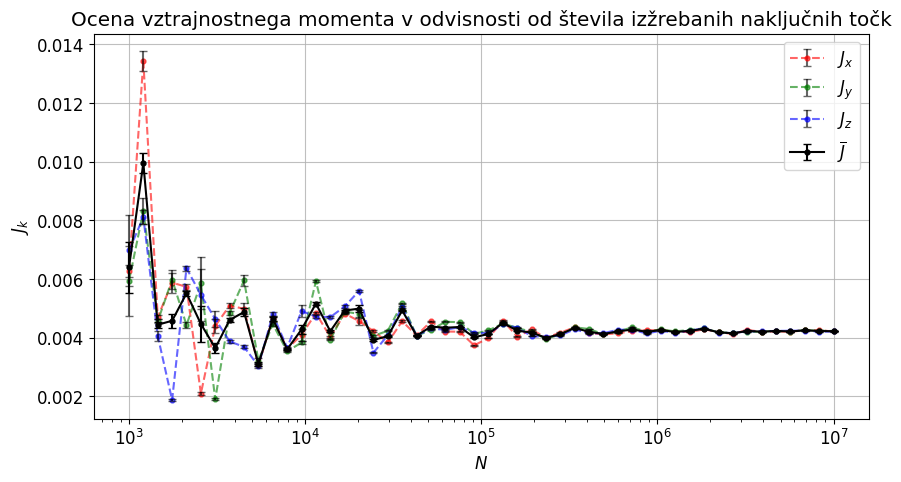
\includegraphics[width=13cm]{telo5.png}
\caption{Ocena za vztrajnostni moment telesa v odvisnosti od števila izžrebanih točk $N$.}
\end{figure}

\subsubsection{Gostita odvisna od radija}

Uvedimo gostoto kot funkcijo radija

\begin{equation}
\rho(r) = r^p,
\end{equation}
kjer je $r$ oddaljenost od koordinatnega izhodišča $r = \sqrt{x^2+y^2+z^2}$ ter $p$ prosti parameter. Pri številu $N=10^7$ izžrebanih točk si poglejmo kako se masa telesa spreminja z vrednostjo parametra $p$. Na sliki 5 je prikazana ocena mase v odvisnosti od vrednosti parametra p pri $N=10^7$ naključnih točkah.

\begin{figure}[h!]
\centering
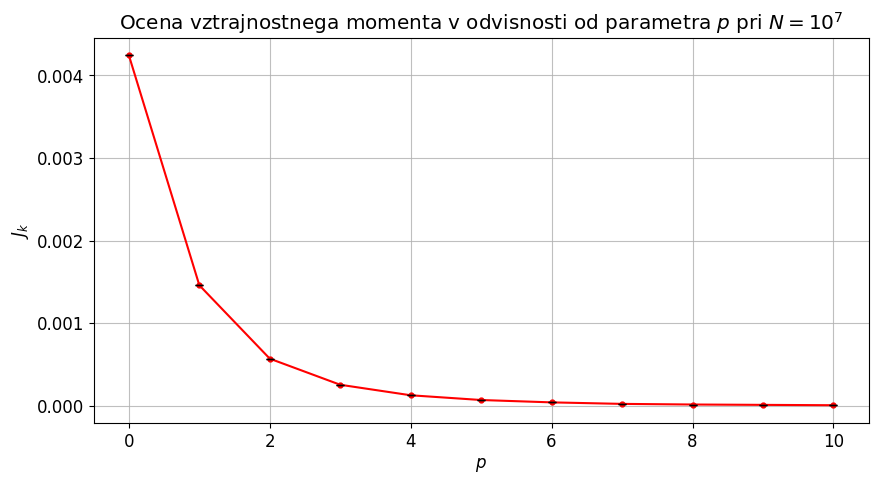
\includegraphics[width=13cm]{telo6.png}
\caption{Ocena vztrajnostnega momenta v odvisnosti od vrednosti parametra p pri $N=10^7$ naključnih točkah.}
\end{figure}
\noindent Vidimo, da vrednost ocene za vztrajnostni moment precej hitro pade, saj je večino volumna telesa blizu koordinatnega izhodišča, kjer je gostota zmeraj manjša za večje vrednosti $p$.


\subsection{Težišče}

Težišče telesa izračunamo po formuli

\begin{equation}
x_{T,k} = \frac{\sum_{i=1}^N \Delta_i \rho(r_i) x_k}{\sum_{i=1}^N \Delta_i \rho(r_i)},
\end{equation}
kjer je $N$ število izžrebanih naključnih točk, $\Delta_i$ ima vrednost $1$, če se točka nahaja v telesu oz. reši neenačbo (2) ter vrednost $0$ sicer, $\rho(r_i)$ gostota v ročki $r_i = (x_i, y_i, z_i)$ in $x_k \in \{x,y,z\}$ koordinata v smeri določene osi.

Težišče smo računali le za primer konstantne gostote $\rho=1$. Na sliki 6 so prikazane koordinate težišča v odvisnosti od števila izžrebanih naključnih točk $N$. Te seveda pravilno konvergirajo k 0, saj je zaradi simetrije telesa težišče v točki $(0,0,0)$.

\begin{figure}[h!]
\centering
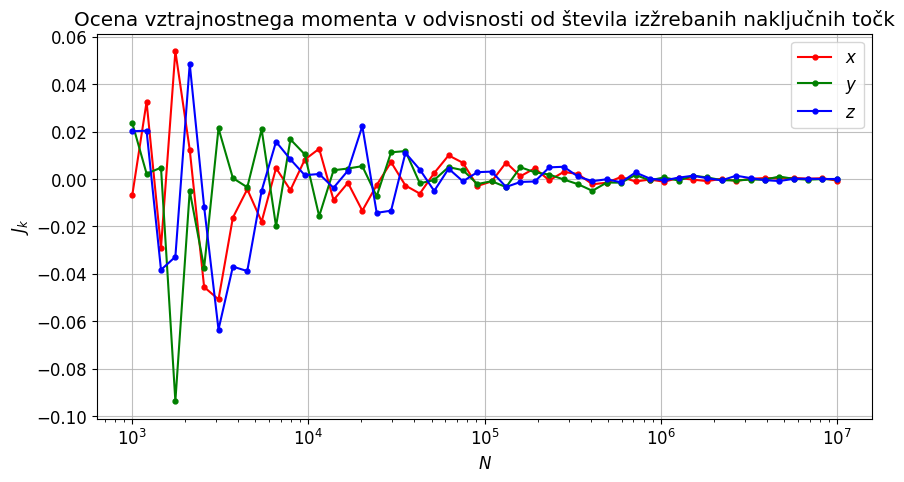
\includegraphics[width=13cm]{telo7.png}
\caption{Ocena za koordinate težišča telesa v odvisnosti od števila izžrebanih točk $N$.}
\end{figure}
\noindent Pri $N=10^7$ izžrebanih točkah pridemo do ocen za koordinate težišča

\[
x_T = -71.1 \cdot 10^{-5} \quad
y_T = -14.6 \cdot 10^{-5} \quad
z_T = -1.7 \cdot 10^{-5} \quad
|r_T| = 72.7 \cdot 10^{-5}.
\]


\section{Transmisivnost krogle}

V enotski krogli se rojevajo žarki $\gamma$. Njihova povprečna prosta pod v snovi, iz katere je krogla, je enaka radiju krogle. Zaradi simetrije krogle lahko poenostavimo problem tako, da se žarki rojevajo le na pozivitnem delu $z$ osi v krogli. Vrednost na $z$ osi pri kateri se naključni $i$-ti žarek rodi označimo z $r_i$. To vrednost žrebamo po porazdelitvi

\[
r_i = \sqrt[3]{\xi_i},
\]
kjer je $\xi_i \in [0,1)$ enakomerno porazdeljeno naključno število. Žarek iz te točke odleti pod naključnim kotom $\theta_i$, ki ga žrebamo po porazdelitvi

\[
\theta_i = \arccos(2\xi_i -1),
\]
kjer je $\xi_i \in [0,1)$ enakomerno porazdeljeno naključno število. Tako ima $\gamma$ žarek, ki se rodi v točki $(0,0,r)$ in nadaljuje svojo pot pod kotom $\theta$ do roba krogle pot

\begin{equation}
d(r,\theta) = -r\cos(\theta) + \sqrt{1-r^2(1-\cos^2(\theta)}.
\end{equation}
Vemo pa, da so dolžine poti žarkov porazdeljene eksponentno v odvisnosti od njihove proste poti $\lambda$. Dolžino poti žarka žrebamo po eksponentni porazdelitvi

\begin{equation}
f_S(s) = \frac{1}{\lambda} e^{-s/\lambda}.
\end{equation}

\subsection{Prosta pot enaka kot radij krogle}

Izračunati želimo transmisivnost enotske krogle za $\gamma$ žarke, ki imajo povprečno prosto pot dolžine 1 $\lambda=1$. Za začetek nastavimo število pobeglih $\gamma$ žarkov $n=0$. Naš algoritem deluje tako, da:

\begin{enumerate}
\item Izžrebamo emisijski kot $\theta_i$ in začetni radij $r_i$.
\item Izžrebamo dolžino poti $s_i$ po eksponentni porazdelitvi
\item Preverimo ali $s_i \geq d(r_i, \theta_i)$. Če to drži je žarek ušel in število $n$ prištejemo $1$.
\end{enumerate}
Točke 1., 2. in 3. $N$ krat ponovimo. Ocena za transmisivnost je nato enaka

\begin{equation}
T = \frac{n}{N}
\end{equation}
in napaka ocene

\begin{equation}
\sigma_T = \frac{1}{N^{3/2}} \sqrt{Nn-n^2}.
\end{equation}

\begin{figure}[h!]
\centering
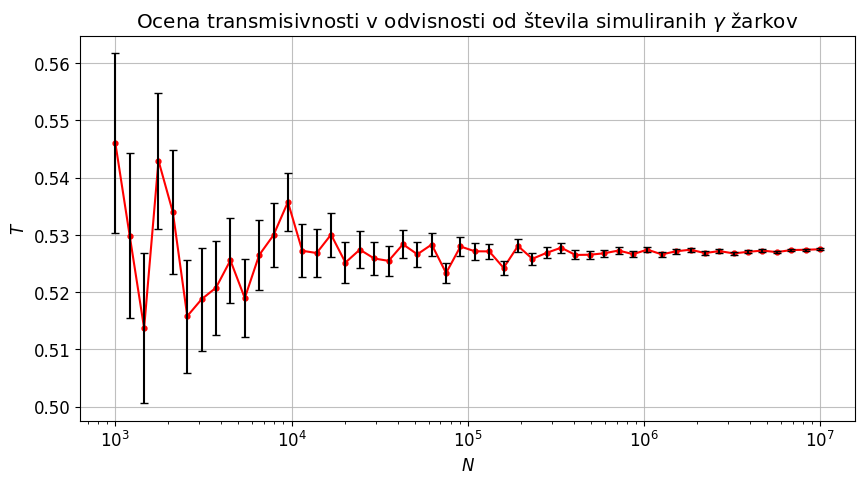
\includegraphics[width=13cm]{gama1.png}
\caption{Ocena transmisivnosti enotske krogle v odvisnosti od števila simuliranih $\gamma$ žarkov $N$.}
\end{figure}
Pri $N=10^7$ simuliranih $\gamma$ žarkih dobimo oceno za transmisivnost pri prosti poti $\gamma$ žarkov $\lambda=1$ oz. enako veliki prosti poti kot radiju krogle

\[
T = 0.5275 \pm 0.0002.
\]

\subsection{Različne proste poti}

V prejšnjem podpoglavju smo izračunali transmisivnost enotske krogle za $\gamma$ žarke s povprečno prosto potjo enako dolgo kot radij krogle. Izračunajmo še transmisivnost enotske krogle za $\gamma$ žarke z različno dolgimi povprečno prostimi potmi. Slika 8 prikazuje transmisivnost enotske krogle v odvisnosti od povprečne proste poti $\gamma$ žarkov. Transmisivnost je izračunana pri $N=10^7$ simuliranih $\gamma$ žarkih. Vidimo, da transmisivnost narašča skupaj z povprečno prosto potjo $\gamma$ žarkov. Transmisivnost počasi konvergija k $1$.

\newpage

\begin{figure}[h!]
\centering
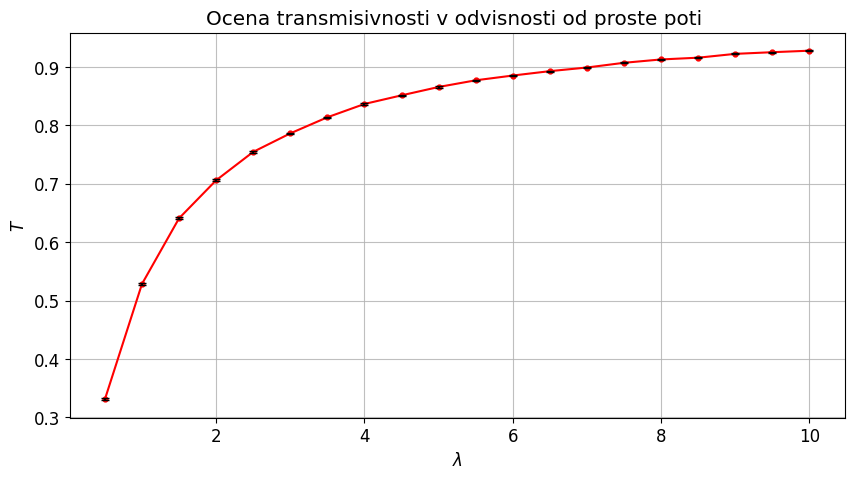
\includegraphics[width=13cm]{gama2.png}
\caption{Ocena transmisivnosti enotske krogle v odvisnosti od povprečne proste poti $\gamma$ žarkov.}
\end{figure}

\section{Model nevtronskega reflektorja}

Tok nevtronov vpada pravokotno na ploščo, v kateri se nevtroni sipljejo in nič ne absorbirajo. Zanima nas porazdelitev po številu sipanj in transmisivnost reflektorja. K reševanju bomo pristopili z eno, dvo in tridimenzionalnim modelom.

V enodimenzionalnem modelu se nevtroni lahko sipajo le naprej ali nazaj in to z isto verjetnostjo. V tem primeru za smer nevtrona žrebamo le med številoma $1$ in $-1$, kjer če izžrebamo število $1$ se nevtron odbije v pozitivno smer in če izžrebamo $-1$ se nevtron odbije v negativno smer. Dolžino njegovega koraka pa žrebamo po eksponentni porazdelitvi

\begin{equation}
f_S(s) = \frac{1}{\lambda} e^{-s/\lambda}.
\end{equation}

V dvodimenzionalnem modelu izžrebamo dolžino koraka nevtrona po porazdelitvi določeno z enačbo (16) in smer nevtrona kot naključni kot odboja $\phi \in [0, 2\pi)$. Nevtroni se tako lahko premikajo po ravnini namesto premici

V tridimenzionalnem modelu poleg dolžine koraka in kota $\phi$ žrebamo še kot $\theta \in [0, \pi)$ in tako nevtronu omogočimo gibanje po celem prostoru.

Reflektor je debel eno enoto. Na začetku nastavimo število pobeglih nevtronov na $n=0$. Naš algoritem deluje tako, da

\begin{enumerate}
\item Izžrebamo vrednost prvega koraka nevtrona $x$ po eksponentni porezdelitvi.
\item Preverimo ali je $x$ koordinata nevtrona večja od debeline reflektorja 1. Če to drži je nevtron ušel in številu $n$ prištejemo 1 ter se vrnemo na točko 1.
\item Preverimo ali je $x$ koordinata nevtrona manjša od 0. Če to drži nevtronu ni uspelo pobegniti in se vrnemo na točko 1.
\item $x$ koordinati nevtrona prištejemo nov korak, katerega dolžina je eksponentno porazdeljena, Žrebanje smeri pa odvisno od dimenzije našega modela. Gremo na točko 2.
\end{enumerate} 
V kodi to seveda napravimo z \texttt{while} zanko, kjer je pogoj za nadaljevanje zanke $x \in (0,1)$. Ko se zanka prekine pogledamo končno vrednost koordinate $x$ nevtrona in vidimo ali se je bil prepuščen ($x>1$) ali odbit ($x<0$).


\subsection{Povprečna prosta pot je polovica debeline plošče}

Izračunati želimo transmisivnost nevtronskega reflektorja z različno dimenzionalnimi modeli pri vrednosti povprečne proste poti nevtrona $\lambda = \frac{1}{2}$ in debelina reflektorja je $d=1$. Na sliki 9 so prikazani rezultati transmisivnosti reflektorja na vse tri modele v odvisnosti od števila simuliranih nevtronov.

\begin{figure}[h!]
\centering
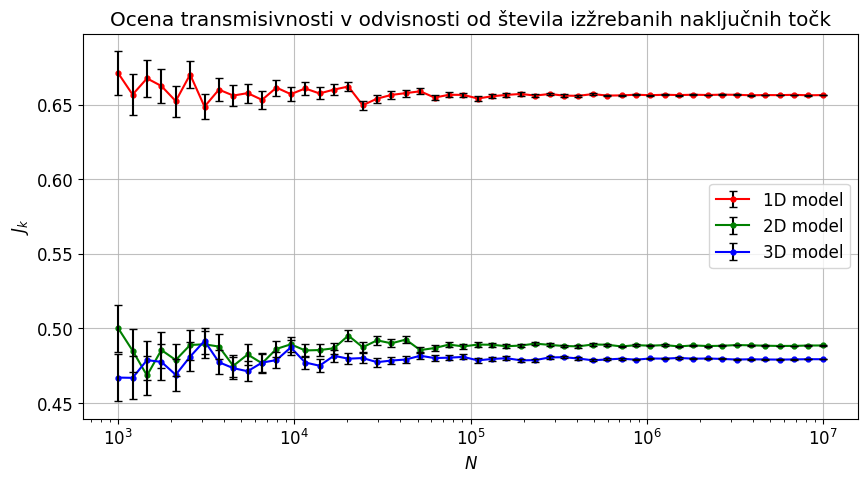
\includegraphics[width=13cm]{nev1.png}
\caption{Ocena transmisivnosti nevtronskega reflektorja za vse tri modele v odvisnosti od števila simuliranih nevtronov $N$.}
\end{figure}
Za nevtrone, ki imajo povprečno prosto pot dolgo $\lambda=1/2$ dobimo pri $N=10^7$ simuliranih nevtronih za oceno transmisivnosti nevtronskega reflektorja rezultate

\[
T_{1D} = 0.6564 \pm 0.0002 \quad
T_{2D} = 0.4885 \pm 0.0002 \quad
T_{3D} = 0.4793 \pm 0.0002.
\]
Vidimo, da transmisivnost z več dimenzijami pada.

Na sliki 10 lahko vidimo porazdelitev nevtronov po številu sipanj za vse tri modele. Simulirali smo $N = 10^7$ nevtronov. Graf je prikazan v logaritemski skali in na ta način lahko vidimo, da je število sipanj porazdeljeno po eksponentni porazdelitvi.

\begin{figure}[h!]
\centering
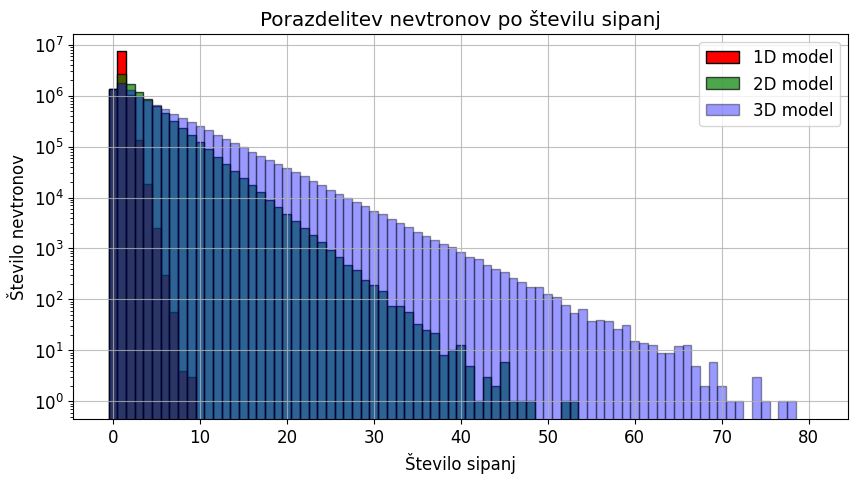
\includegraphics[width=13cm]{nev2.png}
\caption{Porazdelitev nevtronov po številu sipanj.}
\end{figure}
\noindent Po rezultatih lahko vidimo da so se nevtroni v povprečju za vsak model sipali

\[
n_{1D} = 1.0 \quad
n_{2D} = 3.0 \quad
n_{3D} = 4.7.
\]

\subsection{Spreminjamo povprečno prosto pot}

Na sliki 11 lahko vidimo oceno za transmisivnost in povprečno število sipanj nevtronov za vse tri modele v odvisnosti od povprečne proste poti nevtronov. V našem primeru smo vzeli debelino reflektorja enako 1, zato je razmerje med povprečno prosto potjo in debelino reflektorja kar enako vrednosti povprečne proste poti.

\begin{figure}[h!]
\centering
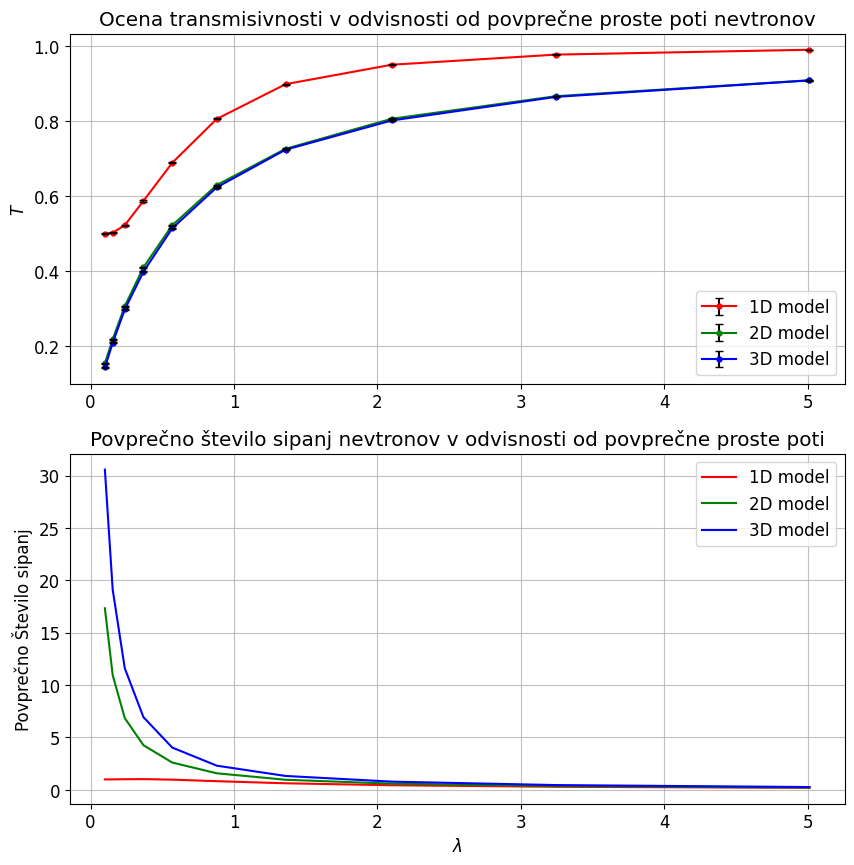
\includegraphics[width=13cm]{nev3.png}
\caption{Ocena za transmisivnost in povprečno število sipanj nevtronov za vse tri modele v odvisnosti od povprečne proste poti nevtronov.}
\end{figure}
\noindent Vidimo, da se z večanjem povprečne proste poti nevtronov veča transmisivnost in niža povprečno število sipanj v vseh modelih.

\section{Zaključek}

Spoznali smo metodo Monte Carlo in z njo rešili več fizikalnih problemov. Metoda temelji na generiranju naključnih števil oz. dogodkov. Več takšnih dogodkov kot generiramo bolj natančen rezultat bo metoda vrnila.

\end{document}